% !TeX root = ../main.tex
\chapter{Curves and line integrals}

\lettrine{C}{urves} have played a part in earlier parts of the course and now we turn our attention to precisely what we mean by this notion.
Up until now we relied more on an intuition, an idea of some type of 1D subset of higher dimensional space.
We will also define how we can integrate scalar and vector fields along these curves.
These types of integrals have a natural and important physical relevance.
We will then study some of the properties of these integrals.
To start let's recall a random selection of curves we have already seen:

\begin{center}
    \begin{tabular}{l l}
        Circle           & \(x^2+y^2 = 4\)                           \\
        Semi-circle      & \(x^2+y^2 = 4\), \(x\geq 0\)              \\
        Ellipse          & \((\frac{x}{2})^2 + (\frac{y}{3})^2 = 4\) \\
        Line             & \(y=5x+2\)                                \\
        Line (in 3D)     & \(x+2y+3z=0\), \(x=4y\)                   \\
        Parabola (in 3D) & \(y=x^2\), \(z=x\)
    \end{tabular}
\end{center}

\noindent
In the above list the curves are written in a way where we are describing a set of points using certain constraint or constraints. In some cases in \emph{implicit} form, in some cases in \emph{explicit} form.
For example, for the circle we formally mean the set  \(\{(x,y):x^2+y^2 = 4\}\).
We have the idea that the curves should be sets which are single connected pieces and we vaguely have an idea that we need curves that are sufficiently smooth.
To proceed we need a precise definition of the 1D objects we can work with.
As part of the definition we force a structure which really allows us to work with these objects in a useful way.

\section{Curves and paths}
Let \(\aalpha : [a,b] \to \bR^n\) be continuous.
In components we write \(\aalpha(t) = (\alpha_1(t),\ldots,\alpha_n(t))\).
We say that \(\aalpha(t)\) is \emph{continuously differentiable} if each component \(\alpha_k(t)\) is differentiable on \([a,b]\) and \(\alpha_k'(t)\) is continuous (Definition~\ref{def:differentiable}).
We say that \(\aalpha(t)\) is \emph{piecewise continuously differentiable} if \([a,b] = [a,c_1]\cup[c_1,c_2] \cup \cdots \cup [c_l,b]\) and \(\aalpha(t)\) is \emph{continuously differentiable} on each of these intervals.

\begin{definition}
    \label{def:path}
    If \(\aalpha: [a,b] \to \bR^n\) is piecewise continuously differentiable then we call it a \emph{path}.
\end{definition}

Note that different functions can trace out the \emph{same} curve in different ways.
Also note that a path has an inherent direction.
We say that this is a \emph{parametric representation} of a given curve.
We already saw examples of paths in Figure~\ref{fig:spiral} and Figure~\ref{fig:particle-circle}.
A few examples of paths are as follows.

\begin{center}
    \begin{tabular}{l l}
        \(\aalpha(t)= (t,t)\),              & \(t\in[0,1]\)                           \\
        \(\aalpha(t) = (\cos t, \sin t)\),  & \(t\in[0,2\pi]\)                        \\
        \(\aalpha(t) = (\cos t, \sin t)\),  & \(t\in [-\frac{\pi}{2},\frac{\pi}{2}]\) \\
        \(\aalpha(t) = (\cos t, -\sin t)\), & \(t\in[0,2\pi]\)                        \\
        \(\aalpha(t)= (t,t,t)\),            & \(t\in[0,1]\)                           \\
        \(\aalpha(t)=(\cos t, \sin t, t)\), & \(t\in [-10,10]\)
    \end{tabular}
\end{center}
\noindent
Observe how some of these parts represent the same circle, perhaps traversed in a different direction.

\section{Line integrals}
Let \(\aalpha(t)\) be a (piecewise continuously differentiable) path on \([a,b]\) and
let \(\ff: \bR^n\to\bR^n\) be a continuous vector field.
Recall that \(\aalpha'(t) = \begin{pmatrix}
    \alpha_1'(t) \\ \vdots \\ \alpha_n'(t)
\end{pmatrix}\)
and \(\ff(\xx) = \begin{pmatrix}
    f_1(\xx) \\ \vdots \\ f_n(\xx)
\end{pmatrix}\).

\begin{definition}[line integral]
    \label{def:line-integral}
    The \emph{line integral} of the vector field \(\ff\) along the path \(\aalpha\) is
    \[
        \int \ff \cdot d\aalpha = \int_{a}^{b} \ff(\aalpha(t)) \cdot \aalpha'(t) \ dt.
    \]
\end{definition}

{Other possible notation:}
\begin{itemize}
    \item  \(\int_C \ff \cdot d\aalpha  \) (if the parametrization of the curve \(C\) is clear);
    \item \(\int f_1 \ d\alpha_1 + \cdots + f_n \ d\alpha_n\) or \(\int f_1 \ dx_1 + \cdots + f_n \ dx_n\).
\end{itemize}





{Example of calculating a line integral}


\begin{example}
    Consider the vector field \(\ff(x,y) := \begin{pmatrix}
        \sqrt y \\ x^3 + y
    \end{pmatrix}\)
    and the path
    \(\aalpha(t):= (t^2,t^3)\), \(t \in (0,1)\).
    Evaluate \(\int \ff \cdot d\aalpha\).
\end{example}
\begin{proof}[Solution]
    \begin{enumerate}
        \item \(\aalpha'(t) = \begin{pmatrix}
                  2t \\ 3t^2
              \end{pmatrix}\);
        \item \(\ff(\aalpha(t)) := \begin{pmatrix}
                  t^{\frac{3}{2}} \\ t^6 + t^3
              \end{pmatrix}\);
        \item \( \ff(\aalpha(t)) \cdot  \aalpha'(t) = \begin{pmatrix}
                  t^{\frac{3}{2}} \\ t^6 + t^3
              \end{pmatrix} \cdot  \begin{pmatrix}
                  2t \\ 3t^2
              \end{pmatrix} = 2 t^{\frac{5}{2}} + 3t^8 + 3t^5\);
        \item
              \(
              \displaystyle\int \ff \cdot d\aalpha = \displaystyle\int_{0}^{1} (2 t^{\frac{5}{2}} + 3t^8 + 3t^5 ) \ dt = \frac{59}{42}.
              \) \qedhere
    \end{enumerate}
\end{proof}


\section{Basic properties}



 {Basic properties of the line integral}
 %    {Combining / dividing paths}
 {Linearity:}
Suppose \(\ff\), \(\gg\) are vector fields and \(\aalpha(t)\) is a path. For any \(c,d\in \bR\),
\[
    \int (c\ff + d\gg) \cdot d\aalpha =  c \int \ff  \cdot d\aalpha +  d \int \gg \cdot d\aalpha.
\]
{Joining / dividing paths:}
Suppose \(\ff\) is a vector field and that
\[
    \aalpha(t) = \begin{cases}
        \aalpha_1(t) & t\in [a,c] \\
        \aalpha_2(t) & t\in [c,b]
    \end{cases}
\]
is a path.
Then
\[
    \int \ff  \cdot d\aalpha = \int \ff  \cdot d\aalpha_1  + \int \ff  \cdot d\aalpha_2.
\]
{Or:}
If we write \(C\), \(C_1\), \(C_2\) for the corresponding curves, then
\[
    \int_{C} \ff  \cdot d\aalpha = \int_{C_1} \ff  \cdot d\aalpha + \int_{C_2} \ff  \cdot d\aalpha.
\]







{Choices of parametrization}

Consider the curve \(C = \{(x,y) : x^2 + y^2 = 1, y\geq 0\}\) (Half circle).

Many possible path parametrization, e.g.,

\begin{itemize}
    \item     \(\aalpha(t):= ( -t , \sqrt{1-t^2})\), \(t\in [-1,1]\)
    \item  \(\bbeta(t) := (\cos t, \sin t)\), \(t\in [0,\pi]\)
\end{itemize}


\begin{definition}[equivalent paths]
    We say that two paths \(\aalpha(t)\) and \(\bbeta(t)\) are \emph{equivalent} if there exists a continuously differentiable function \(u : [c,d] \to [a,b] \) such that \(\aalpha(u(t)) = \bbeta(t)\).
    Furthermore,
    \begin{itemize}
        \item if \(u(c)=a\) and \(u(d)=b\) we say that  \(\aalpha(t)\) and \(\bbeta(t)\) are in the same direction,
        \item if \(u(c)=b\) and \(u(d)=a\) we say that  \(\aalpha(t)\) and \(\bbeta(t)\) are in the opposite direction.
    \end{itemize}
\end{definition}






{Change of parametrization}

\begin{theorem}[Change of parametrization]
    Let \(\ff\) be a continuous vector field and let \(\aalpha\), \(\bbeta\) be equivalent paths.
    Then
    \[
        \int \ff \cdot d\aalpha =
        \begin{cases}
            \int \ff \cdot d\bbeta   & \text{if the paths are in the same direction},     \\
            - \int \ff \cdot d\bbeta & \text{if the paths are in the opposite direction}.
        \end{cases}
    \]
\end{theorem}

\begin{proof}
    \begin{enumerate}
        \item Suppose continuously differentiable path (decomposing if required);
        \item Since \(\aalpha(u(t)) = \bbeta(t)\) chain rule implies that
              \( \bbeta'(t) = \aalpha'(u(t)) \ u'(t)\);
        \item
              \(\displaystyle \int \ff \cdot  d\bbeta = \displaystyle \int_c^d \ff(\bbeta(t)) \cdot \bbeta'(t) \ dt =  \displaystyle \int_c^d \ff(\aalpha(u(t))) \cdot \aalpha'(u(t)) \ u'(t) \ dt \);
        \item Change variables (gives minus if path is opposite direction). \qedhere
    \end{enumerate}
\end{proof}


\section{Applications (gradients / work in physics)}


 {Gradients and line integrals}

\begin{itemize}
    \item Let \(h(x,y)\) be a scalar field in \(\bR^2\);
    \item Recall that the gradient \(\nabla h(x,y)\) is a vector field;
    \item Let \(\aalpha(t)\), \(t\in [0,1]\) be a path;
    \item \(\frac{d}{dt} h(\aalpha(t)) = \nabla h(\aalpha(t))\cdot \aalpha'(t)\);
    \item \[
              \begin{aligned}
                  \int \nabla h \cdot d\aalpha
                   & = \int_0^1 \nabla h(\aalpha(t)) \cdot \alpha'(t)\ dt \\
                   & = \int_0^1 \tfrac{d}{dt} h(\aalpha(t)) \ dt
                  = h(\aalpha(1)) - h(\aalpha(0)).
              \end{aligned}
          \]
\end{itemize}




[Graphic of person walking on a map with contour lines]





{Work in physics 1 (Gravity)}

%{Gravity}

\begin{itemize}
    \item Gravitational field \(\ff(x,y,z) = \left(\begin{smallmatrix}
              0 \\ 0 \\ mg
          \end{smallmatrix}\right)\);
    \item Move particle from \(\aa=(a_1,a_2,a_3)\) to \(\bb=(b_1,b_2,b_3)\) along the path \(\aalpha(t)\), \(t\in [0,1]\);
    \item Work done is defined as \(\int \ff \cdot d\aalpha\).
\end{itemize}

\[
    \begin{aligned}
        \int \ff \cdot d\aalpha & = \int_0^1 \ff(\aalpha(t)) \cdot \aalpha'(t) \ dt
        = \int_0^1 mg \ \alpha_3'(t) \ dt                                               \\
                                & = mg \ \left[ \alpha_3(t)\right]_0^1 = mg(b_3 - a_3).
    \end{aligned}
\]

{I.e.,} work done depends only on the change in height.




    {Work in physics 2 (force field)}

\begin{itemize}
    \item Let \(\ff\) be a force field;
    \item Let \(\xx(t)\) be the position at time \(t\) of a particle moving in the field;
    \item Let \(\vv(t) = \xx'(t)\) be the velocity at time \(t\) of the particle;
    \item Define kinetic energy as \(\frac{m}{2} \norm{\vv(t)}^2\).
\end{itemize}

{Newton's law:}
\(\ff(\xx(t)) = m\xx''(t) = m \vv'(t)\).

    {Work done:}

\[
    \begin{aligned}
        \int \ff \cdot d\xx
         & = \int_0^1 \ff(\xx(t)) \cdot \vv(t) \ dt
        = \int_0^1 m\vv'(t) \cdot \vv(t) \ dt                                   \\
         & = \int_0^1 \tfrac{d}{dt} \left( \tfrac{m}{2} \norm{\vv(t)}^2 \right)
        = \left(  \tfrac{m}{2} \norm{\vv(1)}^2  -  \tfrac{m}{2} \norm{\vv(0)}^2   \right)
    \end{aligned}
\]

{I.e.,}
work done on the particle moving in the force field is equal to the change in kinetic energy.





    {Length of a curve}

Let \(\aalpha(t)\), \(t\in [a,b]\) be a path.
\begin{definition}[length of a curve]
    The length of the piece of the curve between \(\aalpha(a)\) and \(\aalpha(t)\) is defined as
    \[
        s(t) := \int_a^t \norm{\aalpha'(u)} \ du.
    \]
\end{definition}

\begin{itemize}
    \item  \(s'(t) = \norm{\aalpha'(t)} \).
    \item If the path represents a wire and the wire has density \(\varphi(\aalpha(t))\) at the point \(\aalpha(t)\) then the mass of the wire is defined as
          \(M = \displaystyle\int \varphi(\aalpha(t)) \ s'(t) \ dt\).
\end{itemize}







\section{The second fundamental theorem of calculus}



 {The second fundamental theorem of calculus}


 {Recall:}
If \(\varphi:\bR \to \bR\) is differentiable then
\(\int_a^b \varphi'(t) \ dt = \varphi(b) - \varphi(a)\).

\begin{theorem}[2\textsuperscript{nd} fundamental theorem in \(\bR^n\)]
    Suppose that \(\varphi\) is a continuously differentiable scalar field on \(S \subset \bR^n\)
    and suppose that \(\aalpha(t)\), \(t\in[a,b]\) is a path in \(S\).
    Let \(\aa:= \aalpha(a)\),  \(\bb:= \aalpha(b)\).
    Then
    \[
        \int \nabla \varphi \cdot d\aalpha = \varphi(\bb) - \varphi(\aa).
    \]
\end{theorem}

\begin{proof}
    \begin{enumerate}
        \item Suppose that \(\aalpha(t)\) is continuously differentiable;
        \item By the chain rule \(\frac{d}{dt} \varphi(\aalpha(t)) = \nabla \varphi(\aalpha(t))\cdot \aalpha'(t)\);
        \item Consequently \(\int \nabla \varphi \cdot d\aalpha
              = \int_0^1 \nabla \varphi(\aalpha(t)) \cdot \aalpha'(t)\ dt
              = \int_0^1 \tfrac{d}{dt} \varphi(\aalpha(t)) \ dt \)
        \item By 2\textsuperscript{nd} fund.\,theorem in \(\bR\),
              \(\int_0^1 \tfrac{d}{dt} \varphi(\aalpha(t)) \ dt = \varphi(\aalpha(b)) - \varphi(\aalpha(a))\).
    \end{enumerate}
\end{proof}




{Potential energy example}

\begin{itemize}
    \item Earth has mass \(M\) with centre at \((0,0,0)\),
    \item Small particle close to earth has mass \(m\),
    \item Force field of gravitation is equal to
          \(\ff(\xx) := \frac{-GmM}{\norm{\xx}^3}\xx\),
    \item Define potential energy as
          \(\varphi(\xx):= \frac{GmM}{\norm{\xx}}\).
\end{itemize}

We write \(\varphi(x_1,x_2,x_3) = \frac{GmM}{\sqrt{x_1^2 + x_2^2 + x_3^2}}\)
and calculate
\[
    \nabla \varphi(\xx) =
    \begin{pmatrix}
        {(GmM) \ (2x_1)} \ {(-\frac{1}{2}) \ (x_1^2 + x_2^2 + x_3^2)^{-\frac{3}{2}}} \\
        {(GmM) \ (2x_2)} \ {(-\frac{1}{2}) \ (x_1^2 + x_2^2 + x_3^2)^{-\frac{3}{2}}} \\
        {(GmM) \ (2x_3)} \ {(-\frac{1}{2}) \ (x_1^2 + x_2^2 + x_3^2)^{-\frac{3}{2}}}
    \end{pmatrix}
    =   \frac{-GmM}{\norm{\xx}^3}\xx.
\]




\section{The first fundamental theorem of calculus}


 {Connected sets}




\begin{definition}[connected]
    The set \(S\subset \bR^n\) is said to be \emph{connected} if, for every pair of points \(\aa,\bb\in S\), there exists a path \(\aalpha(t), t\in[a,b]\) such that
    \begin{itemize}
        \item \(\aalpha(t)\in S\) for every \( t\in[a,b]\),
        \item \(\aalpha(a)=\aa\) and \(\aalpha(b)=\bb\).
    \end{itemize}
\end{definition}

{Terminology:} Sometimes this is called ``path connected'' to distinguish between different notions.

\colorlet{paleBlue}{blue!10!white}


\begin{figure}
    \begin{tikzpicture}
        \fill[paleBlue] plot [smooth cycle, tension=1] coordinates {(0,0) (1,3) (3,3) (4,1)};
        \fill[white] plot [smooth cycle, tension=1] coordinates {(1,1) (2,1) (2.5,2)};
        \fill[black] (1,2) circle (2pt) node[below]{\(\aa\)};
        \fill[black] (3.8,1) circle (2pt) node[above]{\(\bb\)};
        \draw[] (1,2) -- (.7,2) -- (.7,.2) -- (2.3,.2) -- (2.3,1) -- (3.8,1);
        \node at (1.5,0.5){\(\aalpha(t)\)};
        \node at (1.7,2.5){\(S\)};
    \end{tikzpicture}
    \caption{A connected set.}
\end{figure}







{The first fundamental theorem of calculus}

{Recall:}
If \(f:\bR \to \bR\) is continuous and \(\varphi(x) := \int_a^x f(t) \ dt\) then \(\varphi'(x) = f(x)\).

\begin{theorem}[1\textsuperscript{st} fundamental theorem in \(\bR^n\)]
    Let \(\ff\) be a continuous vector field on a connected set \(S \subset \bR^n\).
    Suppose that, for \(\xx,\aa\in S\), the line integral \(\int \ff \cdot d\aalpha\) is equal for every path \(\aalpha\) such that \(\aalpha(a)=\aa\), \(\aalpha(b)=\xx\).
    Fix \(\aa\in S\) and define \(\varphi(\xx):= \int \ff \cdot d\alpha\).
    Then \(\varphi\) is continuously differentiable and \(\nabla \varphi = \ff\).
\end{theorem}

\begin{proof}[Sketch of proof]
    \begin{enumerate}
        \item As before \(\ee_1 = \left(\begin{smallmatrix}
                  1 \\ 0 \\ 0
              \end{smallmatrix}\right) \),
              \(\ee_2 = \left(\begin{smallmatrix}
                  0 \\ 1 \\ 0
              \end{smallmatrix}\right) \),
              \(\ee_3 = \left(\begin{smallmatrix}
                  0 \\ 0 \\ 1
              \end{smallmatrix}\right) \);
        \item \(\varphi(\xx + h \ee_k) - \varphi(\xx) = \int \ff \cdot d\bbeta_k\) where \(\bbeta_k(t) := \xx + t \ee_k\), \(t\in [0,h]\);
        \item Observe that \(\bbeta'_k(t) = \ee_k\);
        \item \(\frac{\partial \varphi}{\partial x_k} =  \displaystyle\lim_{h\to 0} \frac{1}{h}( \varphi(\xx + h \ee_k) - \varphi(\xx)) = \displaystyle \lim_{h\to 0} \frac{1}{h} \int_0^h \ff(\bbeta_k(t)) \cdot \ee_k \ dt = f_k(\xx)  \);
        \item I.e., \(\nabla \varphi (\xx) =  \ff(\xx)\);
    \end{enumerate}
\end{proof}





{Closed paths}

\begin{definition}[closed path]
    We say a path \(\aalpha(t)\), \(t\in [a,b]\) is \emph{closed} if \(\aalpha(a) = \aalpha(b)\).
\end{definition}



\begin{itemize}
    \item If \(\aalpha(t)\), \(t\in[a,b]\) is a closed path then we can divided it into two paths: Let \(c\in[a,b]\) and consider the two paths \(\aalpha(t)\), \(t\in[a,c]\) and  \(\aalpha(t)\), \(t\in[c,b]\).
    \item Suppose \(\aalpha(t)\), \(t\in [a,b]\) and  \(\bbeta(t)\), \(t\in [c,d]\) are two path starting at \(\aa\) and finishing at \(\bb\). The these can be combined to define a closed path (by following one backward).
\end{itemize}





{Conservative vector fields}

\begin{definition}[conservative vector field]
    A vector field \(\ff\), continuous on \(S \subset \bR^n\) is said to be conservative if there exists a scalar field \(\varphi\) such that, on \(S\), \[\ff = \nabla \varphi.\]
\end{definition}

{Terminology:}

\begin{itemize}
    \item     Some authors call such a vector field a \emph{gradient} (i.e., the vector field is the gradient of some scalar).
    \item If \(\ff = \nabla \varphi\) the \(\varphi\) is called the \emph{potential}.
\end{itemize}

{Non-uniqueness:}
\begin{itemize}
    \item     Observe that \(\nabla \varphi = \nabla(\varphi + C)\) for any constant \(C \in \bR\).
\end{itemize}






{Conservative vector fields}

\begin{theorem}[conservative vector fields]
    The following are equivalent for a vector field \(\ff\):
    \begin{enumerate}
        \item There exists \(\varphi\) such that \(\ff = \nabla \varphi\),
        \item \(\int \ff \cdot d\aalpha\) does not depend on \(\aalpha\), as long as \(\aalpha(a)=\aa\), \(\aalpha(b)=\bb\),
        \item \(\int \ff \cdot d\aalpha = 0\) for any closed path \(\aalpha\).
    \end{enumerate}
\end{theorem}

\begin{proof}
    \begin{description}
        \item[(a) \(\Leftrightarrow\) (b)] We proved in the previous theorems (the two fundamental theorems);
        \item[(b) \(\Rightarrow\) (c)] Let \(\aalpha(t)\) be a closed path and let \(\bbeta(t)\) be the same path in the opposite direction. Observe that \(\int \ff \cdot d\aalpha = - \int \ff \cdot d \bbeta\) but that \(\int \ff \cdot d \aalpha = \int \ff \cdot d \bbeta\) and so \(\int \ff \cdot d \aalpha = 0\);
        \item[(b) \(\Leftarrow\) (c)] The two paths between \(\aa\) and \(\bb\) can be combined (with a minus sign) to give a closed path.
    \end{description}
\end{proof}






{Mixed partial derivatives}

\begin{theorem}
    Suppose that \(\ff\) is a continuously differential vector field.
    If \(\ff = \nabla \varphi\) for some scalar field \(\varphi\) then, for each \(l,k\),
    \[
        \frac{\partial f_l}{\partial x_k} = \frac{\partial f_k}{\partial x_l}.
    \]
\end{theorem}

{Notation:} Here we write, as usual, \(\ff(x_1,\ldots,x_n) = \left(\begin{smallmatrix}
        f_1(x_1,\ldots,x_n)\\
        \vdots \\
        f_n(x_1,\ldots,x_n)
    \end{smallmatrix}\right)\).

\begin{proof}
    By assumption the second order partial derivatives exist and so
    \[
        \tfrac{\partial f_l}{\partial x_k}
        = \tfrac{\partial^2 \varphi}{\partial x_k \partial x_l}
        = \tfrac{\partial^2 \varphi}{\partial x_l \partial x_k}
        = \tfrac{\partial f_k}{\partial x_l}. \qedhere
    \]
\end{proof}

{Useful:}
If a pair of mixed derivatives is not equal then \(\ff\) is \emph{not} conservative.




\section{Potential functions and conservative vector fields}


 {Constructing a potential}

 {Question:}
Suppose we are given a vector field \(\ff\) and we know that \(\ff = \nabla \varphi\) for some \(\varphi\).
How can we calculate \(\varphi\)?

{Two methods:}
\begin{enumerate}
    \item by line integral;
    \item by indefinite integrals.
\end{enumerate}










{Constructing a potential by line integral}






\begin{enumerate}
    \item Suppose that \(\ff\) is a conservative vector field on the rectangle \([a_1,b_1]\times [a_2,b_2]\);
    \item We will define \(\varphi(\xx)\) as the line integral \(\int \ff \cdot d\aalpha\) where \(\aalpha\) is a path between \(\aa=(a_1,a_2)\) and \(\xx\);
    \item For any \(\xx = (x_1,x_2) \in \bR^2\) consider the two paths:
          \begin{itemize}
              \item[H:] \(\aalpha_1(t) := (t,a_2)\), \(t\in [a_1,x_1]\);
              \item[V:]  \(\aalpha_2(t) := (x_1,t)\),  \(t\in [a_2,x_2]\);
          \end{itemize}
\end{enumerate}




\begin{figure}
    \begin{tikzpicture}
        \draw[step=1cm,gray,very thin] (-0.4,-0.4) grid (5.4,3.4);
        \draw[thick,->] (-0.4,0) -- (5.4,0); % node[anchor=north]{\(x_1\)};
        \draw[thick,->] (0,-0.4) -- (0,3.4); % node[anchor=east]{\(x_2\)};
        \draw[fill, blue] (1,1) circle [radius=1.5pt];
        \node[below] at (1,1) {\(\aa\)};
        \draw[fill, blue] (4,3) circle [radius=1.5pt];
        \node[right] at (4,3) {\(\xx\)};
        \draw[->, very thick] (1,1) -- (4,1) node[black,midway,below]{\(\aalpha_1\)};
        \draw[->, very thick] (4,1) -- (4,3) node[black,midway,left]{\(\aalpha_2\)};
        \draw[thick] (1,0) -- (1,-.1) node[below] {\(a_1\)};
        \draw[thick] (4,0) -- (4,-.1) node[below] {\(x_1\)};
        \draw[thick] (0,1) -- (-.1,1) node[left] {\(a_2\)};
        \draw[thick] (0,3) -- (-.1,3) node[left] {\(x_2\)};
    \end{tikzpicture}
    \caption{The paths \(\aalpha_1\) and \(\aalpha_2\).}
\end{figure}





\begin{enumerate}
    \item[4.] Let \(\aalpha(t)\) denote the combination of the two paths;
    \item[5.] Calculate \(\int \ff \cdot d\aalpha = \int_{a_1}^{x_1} \ff(\aalpha_1(t))\cdot \aalpha_1'(t) \ dt +  \int_{a_2}^{x_2} \ff(\aalpha_2(t))\cdot \aalpha_2'(t) \ dt \);
    \item[6.] And so \(\varphi(\xx)  = \int_{a_1}^{x_1} f_1(t,a_2)\ dt + \int_{a_2}^{x_2} f_2(x_1,t)\ dt \).
\end{enumerate}




{Constructing a potential by indefinite integrals}

\begin{enumerate}
    \item Again suppose that \(\ff = \nabla \varphi\) for some scalar field \(\varphi(x,y)\) which we wish to find;
    \item Observe that \(\frac{\partial \varphi}{\partial x} = f_1\) and  \(\frac{\partial \varphi}{\partial y} = f_2\);
    \item  This means that (\(A(y)\), \(B(x)\) are constants of integration)
          \[
              \int_{a}^{x} f_1(t,y) \ dt + A(y) = \varphi(x,y) =  \int_{b}^{y} f_2(x,t) \ dt + B(x);
          \]
    \item Calculating and comparing we can obtain a formula for \(\varphi(x,y)\).
\end{enumerate}


\colorlet{halfBlue}{blue!50!white}
\begin{example}
    Find a potential for \(\ff(x,y) = \left(\begin{smallmatrix}
        e^x y^2 + 1\\ 2e^x y
    \end{smallmatrix}\right)\) on \(\bR^2\).
    \begin{itemize}
        \item \({\color{halfBlue} \int_{a}^{x} f_1(t,y) \ dt + A(y) = } \ e^x y^2 + x + A(y) = \varphi(x,y)\);
        \item \( {\color{halfBlue} \int_{b}^{y} f_2(x,t) \ dt + B(x) = }  e^x y^2 + B(x) = \varphi(x,y) \);
        \item we can choose \(A(y) = 0\) and \(B(x)=x\) to obtain equality above;
        \item potential is \(\varphi(x,y) = e^x y^2 + x\).
    \end{itemize}
\end{example}




{Convex sets}


\begin{definition}[convex set]
    A set \(S\subset \bR^n\) is said to be \emph{convex} if for any \(\xx,\yy\in S\) the segment \(\{t\xx + (1-t)\yy, t\in[0,1]\}\) is contained in \(S\).
\end{definition}



\begin{figure}
    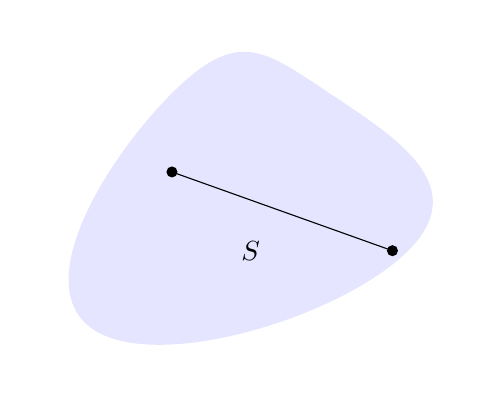
\begin{tikzpicture}
        \fill[paleBlue] plot [smooth cycle, tension=1] coordinates {(0,0) (1,3) (3,3) (4,1)};
        \fill[black] (1,2) circle (2pt) node[below]{\(\xx\)};
        \fill[black] (3.8,1) circle (2pt) node[above]{\(\yy\)};
        \draw[] (1,2) -- (3.8,1);
        \node at (2,1){\(S\)};
    \end{tikzpicture}
    \caption{A convex set.}
\end{figure}


\begin{figure}
    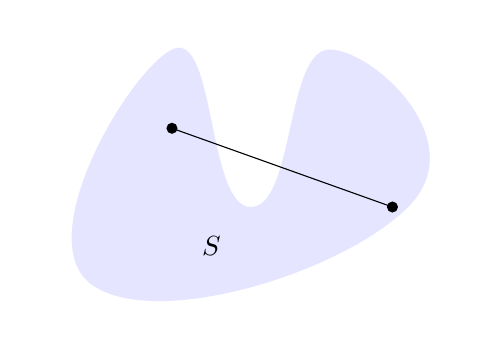
\begin{tikzpicture}
        \fill[paleBlue] plot [smooth cycle, tension=1] coordinates {(0,0) (1,3) (2,1) (3,3) (4,1)};
        \fill[black] (1,2) circle (2pt) node[below]{\(\xx\)};
        \fill[black] (3.8,1) circle (2pt) node[above]{\(\yy\)};
        \draw[] (1,2) -- (3.8,1);
        \node at (1.5,0.5){\(S\)};
    \end{tikzpicture}
    \caption{A set which is not convex.}
\end{figure}







{Sufficient condition for a vector field to be conservative}


\begin{theorem}
    Let\footnote{As usual  \(  f_k(x_1,\ldots,x_n)\) denotes the \(k\)\textsuperscript{th} component of the vector field \(\ff\).} \(\ff\) be a continuously differentiable vector field on a convex region \(S\subset \bR^n\).
    Then \(\ff\) is conservative if and only if
    \[
        \tfrac{\partial f_l}{\partial x_k} = \tfrac{\partial f_k}{\partial x_l},
        \quad \text{for each \(l,k\)}.
    \]
\end{theorem}



\begin{proof}[Sketch of proof]
    \begin{enumerate}
        %\item Already proved that \(\ff\) conservative implies the equality of partial derivatives;
        \item Need only assume \(\partial_g f_l = \partial_l f_k\) and construct a potential;
        \item Let \(\varphi(\xx) = \int \ff \cdot d\aalpha\) where \(\aalpha(t) = t\xx\), \(t\in[0,1]\);
        \item Since \(\aalpha'(t) = \xx\), \(\varphi(\xx) = \int_0^1 \ff(t\xx)\cdot \xx\);
        \item Also (needs proving) \(\partial_k  \varphi(\xx) = \int_{0}^{1} \left( t \partial_k \ff(t\xx) \cdot \xx + f_k(t\xx) \right) \ dt\);
        \item This is equal to \(\int_{0}^{1} \left( t \nabla f_k(t\xx) \cdot \xx + f_k(t\xx) \right) \ dt\) because  \(\partial_g f_l = \partial_l f_k\);
        \item By the chain rule (to \(g(t):= t \nabla f_k(t\xx) \)) this is equal to \(f_k(\xx)\) as required.
    \end{enumerate}

\end{proof}




{Conservative or non-conservative vector field?}


\begin{example}
    Consider the vector field \(\ff(x,y) := \left(\begin{smallmatrix}
        -y (x^2 + y^2)^{-1} \\ x (x^2 + y^2)^{-1}
    \end{smallmatrix}\right)\)
    on \(S = \bR^2 \setminus (0,0)\).
    \begin{enumerate}
        \item Verify that \(  \tfrac{\partial f_2}{\partial y} = \tfrac{\partial f_2}{\partial x}\);
        \item Evaluate the line integral \(\int \ff \cdot d\aalpha\) where \(\aalpha(t) := (a \cos t, a \sin t)\), \(t\in [0,2\pi]\).
    \end{enumerate}

\end{example}


\begin{itemize}
    \item \(S\) is not convex;
    \item Line integral is the same for any circle, independent of the radius.
\end{itemize}


{Evaluation of line integral}


\begin{enumerate}
    \item \(\aalpha'(t) = \left(\begin{smallmatrix}
                  -a \sin t \\ a \cos t
              \end{smallmatrix}\right)\) and \(\ff(\aalpha(t)) = \frac{1}{a^2} \left(\begin{smallmatrix}
                  -a \sin t \\ a \cos t
              \end{smallmatrix}\right)   \);
    \item \(\ff(\aalpha(t)) \cdot \aalpha'(t) = \sin^2 t + \cos^2 t = 1  \);
    \item \(\int \ff \cdot d\aalpha = \int_{0}^{2\pi} (1) \ dt = 2\pi \).
\end{enumerate}



\section{Applications to differential equations}



 {Exact  differential equations {\color{black}{\(p(x,y) + q(x,y) \frac{d y}{d x}=0\)}}}

% Differential equations of the form  \(p(x,y) = q(x,y) \frac{d y}{d x}\).
\begin{theorem}
    \begin{enumerate}
        \item[(a)]         If \(\varphi(x,y)\) satisfies
              \(\nabla \varphi(x,y) =   \left(\begin{smallmatrix}
                      p(x,y) \\ q(x,y)
                  \end{smallmatrix}\right)\)
              then the solution \(y(x)\) of the equation \(p(x,y) = q(x,y) \frac{d y}{d x}\) satisfies \(\varphi(x,y(x))=C\) for some \(C\in \bR\).
        \item[(b)] Conversely, if  \(\varphi(x,y(x))=C\)  defines implicitly a function \(y(x)\), then \(y(x)\) is a solution to the equation  \(p(x,y) = q(x,y) \frac{d y}{d x}\).
    \end{enumerate}
\end{theorem}

\begin{proof}
    \begin{enumerate}
        \item If \(y(x)\) satisfies  \(\varphi(x,y(x))=C\), then by the chain rule and \(\nabla \varphi =   \left(\begin{smallmatrix}
                  p \\ q
              \end{smallmatrix}\right)\), \(p(x,y(x)) + y'(x) q(x,y(x)) = 0\);
        \item Conversely, if \(y(x)\) is a solution, \(\varphi(x,y(x))\) must be constant in \(x\). \qedhere
    \end{enumerate}
\end{proof}

\begin{example}
    Solve \(y^2 + 2xyy' = 0\).
    Let \(p(x,y) = y^2\), \(q(x,y) = 2xy\) and find \(\varphi(x,y) = xy^2\) so \(\nabla \varphi = \left(\begin{smallmatrix}
            p\\ q
        \end{smallmatrix}\right)\).
    Solutions satisfy \(\varphi(x,y(x))= x y(x)^2 =C\), i.e., \(y(x) = \sqrt{\frac{C}{x}}\).
\end{example}